%%
%% Copyright (c) 2018-2019 Weitian LI <liweitianux@sjtu.edu.cn>
%% Creative Commons BY 4.0
%%

\chapter{绪论}
\label{chap:introduction}

%=====================================================================
\section{研究背景}

理解宇宙的结构、起源和演化,是人类孜孜不倦地追求的目标,在哲学和科学中占据重要地位.
经过几代人的努力,宇宙学的\ac{bbt}终于得以建立.
该理论已被大量观测证据所支持,比如星系的红移--距离关系(即 Hubble 定律)、
\ac{cmb}辐射、星系的大尺度分布规律、早期元素丰度、等等,
是目前宇宙学的标准模型.

根据大爆炸宇宙学模型,宇宙起源于约 138 亿年前的一次大爆炸,然后随着宇宙的膨胀,
温度以及能量密度都逐渐降低,宇宙主要经历了\ac{inflation}、\ac{bbn}、
\ac{recombination}、\ac{da}、\ac{reionization}、
形成星系及大尺度结构等阶段,如\autoref{fig:univ-history} 所示.

\begin{figure}[htp]
  \centering
  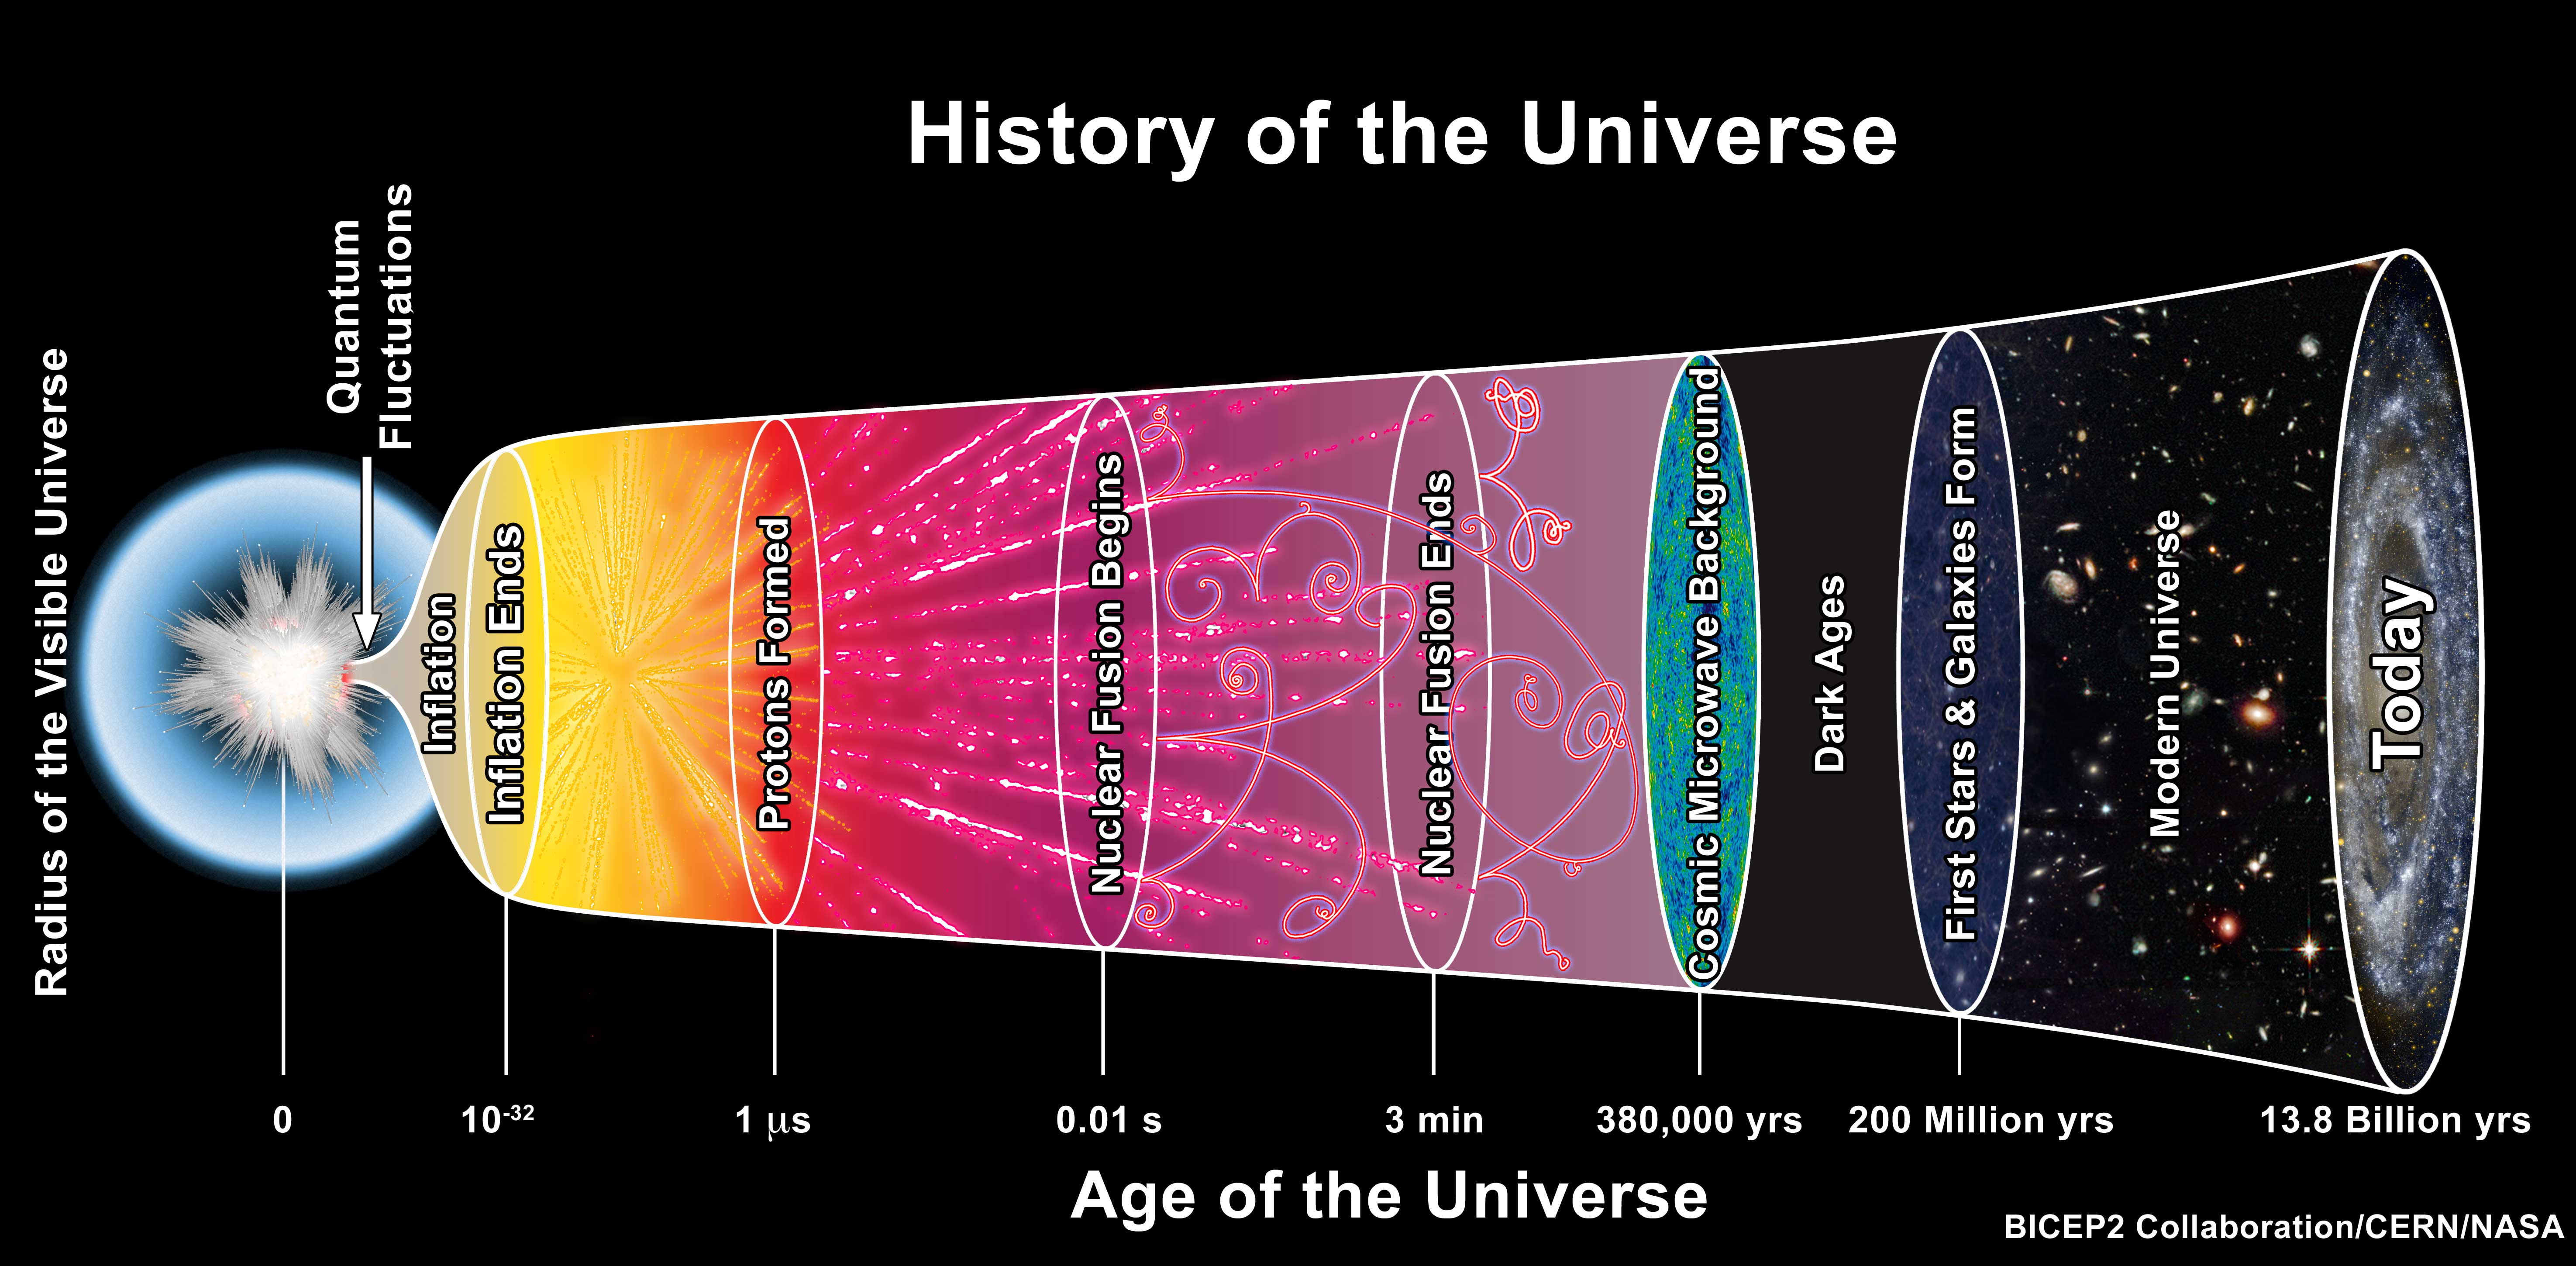
\includegraphics[width=\textwidth]{universe-history}
  \bicaption[宇宙的演化历史]{%
    宇宙从大爆炸到今天的演化历史.
  }{%
    The evolution of the Universe from the Big Bang
    to the present.
    \\来源/Credit:
    \ac{bicep}2/\ac{cern}/\ac{nasa}; \ac{cc}0 1.0.
  }
  \label{fig:univ-history}
\end{figure}

大爆炸之后约 40 万年,宇宙冷却至大约 \SI{3000}{\kelvin},
自由电子与离子结合形成中性原子,于是光子与重子物质脱耦,
并开始在宇宙中自由传播,形成弥漫于整个宇宙的背景辐射,即 \ac{cmb} 辐射.
但是,此时尚未形成发光天体,因此宇宙进入了\ac{da}.
随着物质的密度扰动在引力作用下增长,第一代天体开始形成并产生辐射,
使得中性的重子物质再次被逐步电离,宇宙从此结束\ac{da}并走入\ac{eor}.
随着各尺度上的天体结构的逐步形成与演化,重子物质被充分电离,宇宙也演化形成今天的格局.

\begin{figure}[htp]
  \centering
  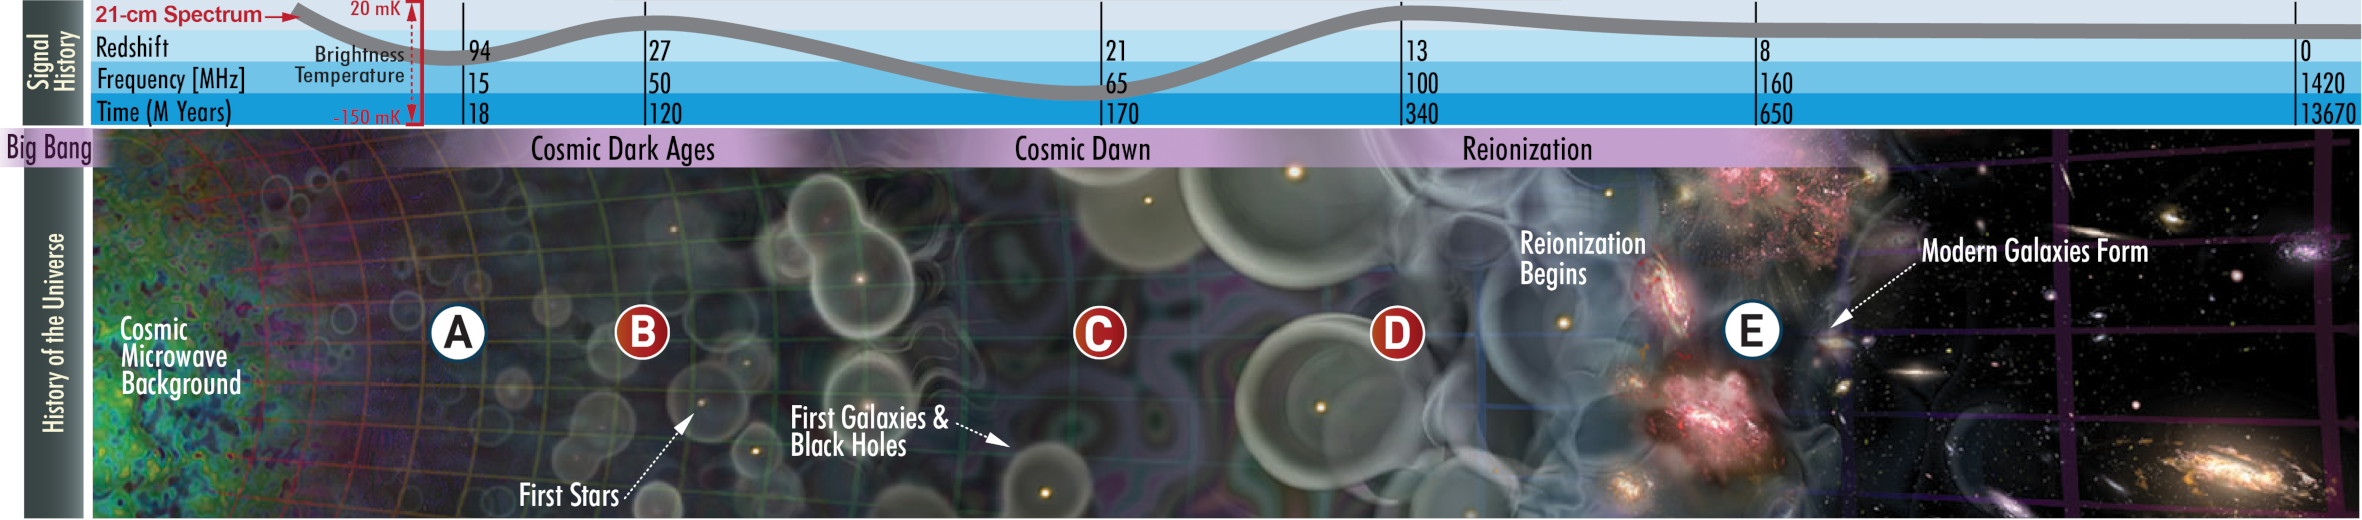
\includegraphics[width=\textwidth]{cosmic-stages-dare}
  \bicaption[宇宙的黑暗时期与再电离时期示意图]{%
    宇宙的黑暗时期与再电离时期示意图,其中显示了\acs*{aoi} (A)、\acs*{da} (B)、
    \acs*{cd} (C) 以及再电离时期 (D, E).
    上方的曲线显示了理论预测的 EoR 信号的强度.
  }{%
    A schematic showing the Dark Ages and the EoR of the Universe,
    mainly including the \acl*{aoi} (A),
    the \acl*{da} (B), the \acl*{cd} (C), and the EoR (D, E).
    The thick curve in the top panel shows the predicted intensity
    of the EoR signal.
    \\来源/Credit:
    \acs{dare},
    \url{http://lunar.colorado.edu/dare/science.html}, (2018-09-23).
  }
  \label{fig:cosmic-stages}
\end{figure}

我们已借助多波段观测掌握了大量有关宇宙近期演化
($\ac{redshift} \lesssim 6$;宇宙已充分电离之后)的信息;
通过研究 \ac{cmb},我们对宇宙的早期历史
($\ac{redshift} \gtrsim 1100$;自由电子\ac{recombination}之前)有了深刻理解.
然而,我们对中间的那段时期($\ac{redshift} \sim \numrange{6}{1100}$)却知之甚少.
这段时期可细分为以下四个阶段\cite{koopmans2015}:
\acs{aoi} (\acl{aoi}; $\ac{redshift} \sim \numrange{200}{1100}$)、
\acs{da} ($\ac{redshift} \sim \numrange{30}{200}$)、
\acs{cd} (\acl{cd}; $\ac{redshift} \sim \numrange{15}{30}$)
以及\acl{eor} ($\ac{redshift} \sim \numrange{6}{15}$),
如\autoref{fig:cosmic-stages} 所示.
对于其中距离我们相对较近的\acl{eor},
我们目前仅获得非常有限的间接观测信息,比如:
该时期的\ac{hi}对高红移\ac{quasar}的 Lyα 吸收 \cite{becker2001}、
该时期的自由电子对 \ac{cmb} 光子的 Thomson 散射 \cite{kaplinghat2003}.
但是,我们仍然缺乏来自\acl{eor}的直接观测证据,
对该时期的基本性质和关键物理过程仍不清楚,比如:
第一代天体是何时以及如何形成的?
主要的电离源有哪些以及它们是如何影响再电离过程的?
\ac{hii}区的尺度以及演化过程如何?
研究\acl{eor}的对于理解宇宙早期结构形成以及星系的形成与演化有重要意义,
是建立完整的宇宙演化图景的关键环节之一.
具体请参见 \citeay{fan2006}, \citeay{morales2010},
\citeay{pritchard2012}, \citeay{zaroubi2013},
\citeay{koopmans2015}, \citeay{mcQuinn2016} 等综述文.

在\acl{eor}及其之前的\ac{da},尽管缺乏发光天体可供观测,
但是宇宙中丰富的\ac{hi}所辐射的 \ac{21cmline}
(以下简称 \emph{21\,cm 信号};详见 \autoref{sec:eor-signal})
为直接探测该时期提供了一条有效途径.
对 21\,cm 信号的探测是目前对\acl{eor}及其之前的\ac{da}开展系统性
研究的最直接而有效的观测手段
\cite{madau1997,tozzi2000,furlanetto2006,koopmans2015,furlanetto2016}.

\ac{hi} \ac{21cmline}的本征频率约为 \SI{1420}{\MHz}.
源自再电离时期的 21\,cm 信号(以下简称 \emph{EoR 信号})经历显著红移后
应出现在约 \SIrange{90}{200}{\MHz},对应于低频射电波段.
EoR 信号到达地球时已非常微弱,亮温度仅约几 \si{\mK} 至十几 \si{\mK},
因此需要具有极高灵敏度的低频观测设备才能捕获该信号,比如大规模低频干涉阵列.
目前已建成或正在建设的干涉阵列主要有:
\ac{21cma} \cite{zheng2016}、
\ac{gmrt} \cite{paciga2011}、
\ac{mwa} \cite{bowman2013,tingay2013}、
\ac{lofar} \cite{vanHaarlem2013}、
\ac{lwa} \cite{ellingson2009}、
\ac{paper} \cite{parsons2010}、
\ac{hera} \cite{deBoer2017}、
\ac{ska} \cite{mellema2013,koopmans2015}.
然而,利用干涉阵列探测 EoR 信号仍面临诸多困难与挑战
\cite{morales2010,wijnholds2010},
其中主要包括:
识别并扣除强烈的前景干扰、扣除人工源的\ac{rfi}、修正电离层的扰动、
苛刻的仪器校准要求、海量数据处理和高动态范围成像.
详见 \autoref{sec:det-difficulties}.

在低频射电波段,强烈的前景干扰(主要源自银河系以及河外点源;
详见 \autoref{sec:fg-intro})比待探测的 EoR 信号高出约 5 个数量级;
即便按干涉阵列所测量的天空亮度涨落来衡量,前景干扰的涨落也是待测信号的数千倍
\cite{zaroubi2013}.
如何准确把握前景干扰并将其扣除,是成功探测 EoR 信号的关键.
由于低频射电波段的观测十分有限,尤其是巡天数据的严重不足
\cite{deOliveiraCosta2008,zheng2017gal},
我们对该波段的前景的了解仍然比较有限,无法达到探测 EoR 信号所要求的精度
\cite{liu2012,harker2015,offringa2016,murray2017,procopio2017}.
因此,我们需要挖掘已有海量的中高频射电观测以及其他多波段观测数据,
并结合逐渐积累的低频观测数据,深入理解低频射电前景辐射,构建并完善前景模型,
为识别并扣除前景干扰提供有力支撑.

尽管前景辐射的频谱在本质上是光滑的,而 EoR 信号的频谱呈锯齿状,
两者具有很好的可区分性 \cite{wang2006,jelic2008,harker2009,wang2013}.
然而在实际情况中,受到干涉阵列的复杂仪器效应、观测干扰、
数据处理技术的限制等多种因素的影响,
前景频谱的光滑性会遭到破坏,导致 EoR 信号的提取变得尤其困难
\cite{liu2009ps,labropoulos2009,gehlot2018,mertens2018}.
因此,研发行之有效的前景处理和 EoR 信号提取算法,亦是当前的重要研究课题
\cite{chapman2016,pober2016,zhang2016,thyagarajan2018}.


%=====================================================================
\section{研究内容}

本文的研究内容分为以下两部分:
\begin{itemize}
\item
\emph{改进星系团射电晕的建模以及评估其对 EoR 探测的影响:}
深刻理解各前景成分的性质(如强度、空间分布、频谱结构)并充分把握它们对 EoR 探测的干扰方式,
是研发具有针对性的前景去除和 EoR 信号分离算法的前提与关键.
在现阶段缺乏足够可用的高质量低频观测数据的情况下,
挖掘已有多波段观测数据并准确模拟低频射电天空,
是开展前景干扰研究以及 EoR 信号分离算法研发的可行办法.

\hspace{2\ccwd}%
在诸多前景成分之中,银河系的弥散辐射 [包括\ac{rad-syn}和\ac{rad-ff}]
以及河外\ac{src-point}辐射是最主要的成分,目前已被广泛地研究
\cite{shaver1999,diMatteo2004,gleser2008,liu2012,murray2017,spinelli2018}.
除此之外,剩下的前景辐射主要来自河外\ac{src-extended},其中包括:
\ac{icm} \cite{feretti2012} 产生的\ac{rh}、\ac{rr}和\ac{rmh}、
\ac{gc}之外的\ac{igm} \cite{keshet2004}、
以及\ac{lsf} \cite{vazza2015}.
对于这些河外\ac{src-extended},已获得的观测证据不多,在低频射电波段更加不足.
关于它们将具体如何影响 EoR 探测,目前的理解非常有限,亟待深入且系统的研究.

\hspace{2\ccwd}%
与其他几类河外\ac{src-extended}相比,\ac{rh}拥有更多的观测证据和理论研究,
这些条件允许我们构建一个更物理、更完善的模型用来模拟\ac{rh}的低频射电辐射,
改进低频射电天空的模拟,
进而在考虑干涉阵列的实际仪器效应的情况下,定量地评估\ac{rh}对 EoR 探测的影响.

%.......................................
\item
\emph{研发 EoR 信号分离新算法:}
为了提取淹没于前景干扰之中的 EoR 信号,一系列方法已被提出来用于处理前景
(详见 \autoref{sec:fg-methods}).
这些前景处理方法可大致分为\ac{fg-rm}和\ac{fg-avd}两大类,
并且都依赖于一个重要前提:前景辐射的频谱必须非常光滑.
据此,这些方法通过构建一个模型来拟合光滑的前景成分并扣除,
或者在功率谱空间尽量避开前景污染区域,
从而提取出微弱的 EoR 信号 \cite{chapman2016}.

\hspace{2\ccwd}%
然而在实际情况中,干涉阵列的\ac{beam}存在频率依赖效应(以下简称\emph{波束效应}),
即\ac{beam}的形状随观测频率而变化,因此前景辐射源会产生沿频率方向快速变化的涨落,
严重破坏前景频谱的光滑性 \cite{liu2009ps},
导致现有\ac{fg-rm}方法难以区分前景干扰与 EoR 信号,
从而无法有效地分离 EoR 信号(详见 \autoref{sec:beam-effect}).

\hspace{2\ccwd}%
考虑到干涉列阵的\ac{beam}的形状非常复杂,为现有方法打造一个实际可用的模型
用以克服上述复杂的波束效应将非常困难 \cite{lochner2015},
因此基于\ac{dl}研发 EoR 信号分离新算法是一条更加可行且具有吸引力的途径
\cite{herbel2018,vafaeiSadr2019},
通过从数据中学习知识并自适应地优化自身模型,
从而达到克服波束效应并分离 EoR 信号的目标.

\end{itemize}

本文的研究目标是:
(1)改进\ac{rh}的模拟,考虑干涉阵列的实际仪器效应,
获得更精细、更符合实际的低频射电天空的模拟图像,
进而有效地评估\ac{rh}对 EoR 探测的影响.
(2)基于\ac{dl},研发能够有效克服干涉阵列的波束效应的 EoR 信号分离新算法,
并运用到上述模拟数据进行测试和优化.


%=====================================================================
\section{研究方案}

本文遵循以下主要步骤开展工作,完成研究内容,达到研究目标:
\begin{enumerate}
\item
调研\ac{rh}的相关理论研究和观测证据,理解其形成机制和演化规律,
构建模型并模拟\ac{rh}在低频射电波段的\ac{skymap}.
搜集\ac{rh}的现有观测数据,约束模型参数,获得可靠的模拟结果.

\item
采用 SKA1-Low 干涉阵列的布局方案,对上一步所得的\ac{skymap}开展模拟观测,
得到\ac{vis}数据并成像,获得高仿真的\enquote{观测}图像.
通过这种模拟,干涉阵列的复杂仪器效应(如本文涉及的波束效应)得以有效地整合到研究流程之中.

\item
基于上述模拟所得的\enquote{观测}图像,利用一维和二维\ac{ps},
对比\ac{rh}和EoR 信号的异同,
量化\ac{rh}在运用\ac{fg-rm}或\ac{fg-avd}方法的情况下对 EoR 探测的影响,
充分评估\ac{rh}作为前景干扰成分的重要程度.

\item
调研目前主流的\ac{dl}算法,筛选出适用于 EoR 信号分离的算法并加以必要的改进,
利用上述模拟数据对算法进行训练和调优,充分说明新算法的可行性和优势.

\end{enumerate}


%=====================================================================
\section{本文框架}

本文余下章节安排如下:
\autoref{chap:radio-astronomy}将介绍射电天文学和射电干涉技术的基础知识,
主要包括基本辐射理论、天线原理、干涉成像技术等.
在\autoref{chap:detection},我们将介绍利用\ac{hi} 21\,cm 信号
探测宇宙再电离时期的主要方法、面临的困难、以及前景处理方法.
在\autoref{chap:simulation},我们首先模拟各前景成分和 EoR 信号的\ac{skymap},
然后进行干涉阵列的模拟观测,得到整合了实际仪器效应的\enquote{观测}图像.
据此,我们在\autoref{chap:halo}借助\ac{ps}量化评估\ac{rh}对
EoR 探测的具体影响.
\autoref{chap:cdae}将阐述我们提出的基于\ac{dl}的 EoR 分离新算法并演示其效果.
最后,我们对全文进行总结并简要展望.

全文采用一个由 \lcdm/ 模型描述的平直宇宙,参数为:
$\acs{H0} = 100\,\acs{h}\,\si{\km\per\second\per\Mpc}
= \SI{71}{\km\per\second\per\Mpc}$,
$\acs{Om0} = 0.27$,
$\acs{Ol0} = 1 - \acs{Om0} = 0.73$,
$\acs{Ob0} = 0.046$,
$\acs{ns} = 0.96$ 以及 $\acs{sigma8} = 0.81$.
如无额外说明,本文给出的误差对应 68\% 的置信水平;
使用的幂律谱形式为 $\acs{S-nu} \propto \acs{freq}^{-\acs{spec-index}}$,
其中 \acs{S-nu} 为\acl{S-nu}, \acs{spec-index} 为\acl{spec-index}.
本文使用的中文术语遵循\href{%
  http://astrodict.china-vo.org/
}{英汉天文学名词数据库}\footnote{%
  英汉天文学名词数据库:
  \url{http://astrodict.china-vo.org/}}
以及 Google 的\href{%
  https://developers.google.com/machine-learning/glossary/?hl=zh-CN
}{机器学习术语表}\footnote{%
  机器学习术语表:
  \url{https://developers.google.com/machine-learning/glossary/?hl=zh-CN}}.


%% EOF
